\begin{abstract}
Decision forests, including random forests and gradient boosting trees, remain the leading machine learning methods for many real-world data problems, specifically on tabular data.
However, current standard implementations only operate in batch mode, and therefore cannot incrementally update when more data arrive. 
Several previous works developed streaming trees and ensembles to overcome this limitation. Nonetheless, we found that those state-of-the-art algorithms suffer from a number of drawbacks, including performing very poorly on some problems and requiring a huge amount of memory on others. 
We therefore developed the simplest possible extension of decision trees we could think of: given new data, simply update existing trees by continuing to grow them, and replace some old trees with new ones to control the total number of trees. 
On three standard datasets, we illustrate that our approach, \textit{Stream Decision Forest} (SDF), does not suffer from either of the aforementioned limitations. 
In a benchmark suite containing 72 classification problems (the OpenML-CC18 data suite), we illustrate that our approach often performs as well, and sometimes better even, than the batch mode random forest algorithm. 
Thus, we believe SDFs establish a simple standard for streaming trees and forests that could readily be applied to many real-world problems, including those with distribution drift and continual learning.
\end{abstract}

\section{Introduction}
\label{introduction}
In recent decades, machine learning methods facilitate the utilization of modern data and make scientific progress in health care, technology, commerce, and more \citep{jordan_machine_2015}. 
Among those methods, decision forests, such as random forests (RFs) and gradient boosting trees (GBTs) are the leading strategies for batch tasks like classifications, outperforming all others on real-world datasets and machine learning competitions \citep{breiman_random_2001, caruana_empirical_2006, caruana_empirical_2008, fernandez-delgado_we_2014, chen_xgboost_2016}.
However, training forests with continuous inputs poses new challenges for these estimators.
Larger sample sizes often require overwhelmingly more computational time and space, and different scenarios of streaming inputs would need flexible strategies for model updates \citep{liu_isolation_2008, abdulsalam_streaming_2007}. This means that, for batch tree estimators like RFs, all available sample data must be stored, and refitting everything is needed for each model update \citep{amit_shape_1997, breiman_random_2001}. Even with enough computational resources to do so, out-of-distribution (OOD) problems could still undermine the validity of older data \citep{geisa_towards_2021}. Moreover, learning scenarios like continual learning involve data from multiple tasks, representing a particular challenge for model updates \citep{van_de_ven_three_2019}.

By incrementally updating the estimators with indefinite batches of new training samples, streaming trees can continuously optimize the tree structures without storing old data \citep{domingos_mining_2000, bifet_adaptive_2009, lakshminarayanan_mondrian_2014, ben-haim_streaming_2010}. Furthermore, in forest ensembles, older trees could be pruned to keep up with the current data distribution. Attempts have been made to adapt decision trees (DTs) to streaming tasks, including Hoeffding trees (HTs) and Mondrian forests (MFs) \citep{domingos_mining_2000, lakshminarayanan_mondrian_2014}. These two state-of-the-art algorithms have been tested in many synthetic and real-world scenarios \citep{pfahringer_new_2007, gomes_machine_2019, lakshminarayanan_mondrian_2016, khannouz_benchmark_2020}. Nonetheless, we find them performing poorly in certain tasks and using excessive memories on large datasets, which significantly restrict their applications.

In this paper, we explore the simplest incremental update method to extend a fitted decision tree and introduce our streaming tree implementations: \textit{Stream Decision Tree} (SDT) and \textit{Stream Decision Forest} (SDF).
After the initial fitting, an SDT takes every new batch of training samples and splits its leaf nodes when the criteria are met. SDFs ensemble SDTs with bootstrapping and replace old trees with new ones to control the total number of estimators. 
On three standard datasets with varying complexities, we compare the performance of streaming and batch estimators and illustrate the consistently high performance of SDFs without the aforementioned limitations of HTs and MFs. Then in the OpenML-CC18 benchmark suite,\footnote{\url{https://www.openml.org/s/99}} which contains 72 diverse classification tasks, we demonstrate that SDFs often achieve accuracy similar to, sometimes even better than, those of batch mode RFs \citep{vanschoren_openml_2013, bischl_openml_2019}. Overall, we believe our simplest approach to streaming trees could be readily applied to many real-world problems, including OOD problems and continual learning \citep{geisa_towards_2021, van_de_ven_three_2019}.

\section{Methods} 
\label{methods}

\subsection{Streaming Trees}
\begin{algorithm}[!htb]
\caption{Incrementally update a decision tree with a batch of training samples.}
\label{alg:sdt}
\begin{algorithmic}[1]
\Require 
\Statex (1) $T$ \Comment{current tree}
\Statex (2) $\mathcal{D}_n = (\mathbf{x},\mathbf{y}) \in \mathbb{R}^{n \times p} \times \{1,\ldots, K\}^n$ \Comment{batch of training samples}
\Statex (3) split criteria \Comment{e.g., minimum node size}
\Ensure
$T$ \Comment{updated tree}
\Function{SDT.update\_tree}{$T,\mathbf{x},\mathbf{y}$}
\For{each $i \in [n]$}
\State find the leaf node $x_i$ would fall into
\State label that leaf node as a ``false root''
\State update index set for this leaf node to include $i$
\EndFor
\For{each ``false root''}
% \State update the node with associated samples
\State split the node if satisfying split criteria
\For{both child nodes}
\State mark as ``false roots''
\EndFor 
\EndFor
\State \Return $T$
\EndFunction 
\end{algorithmic}
\end{algorithm}

\begin{figure*}[!htb]
\centering
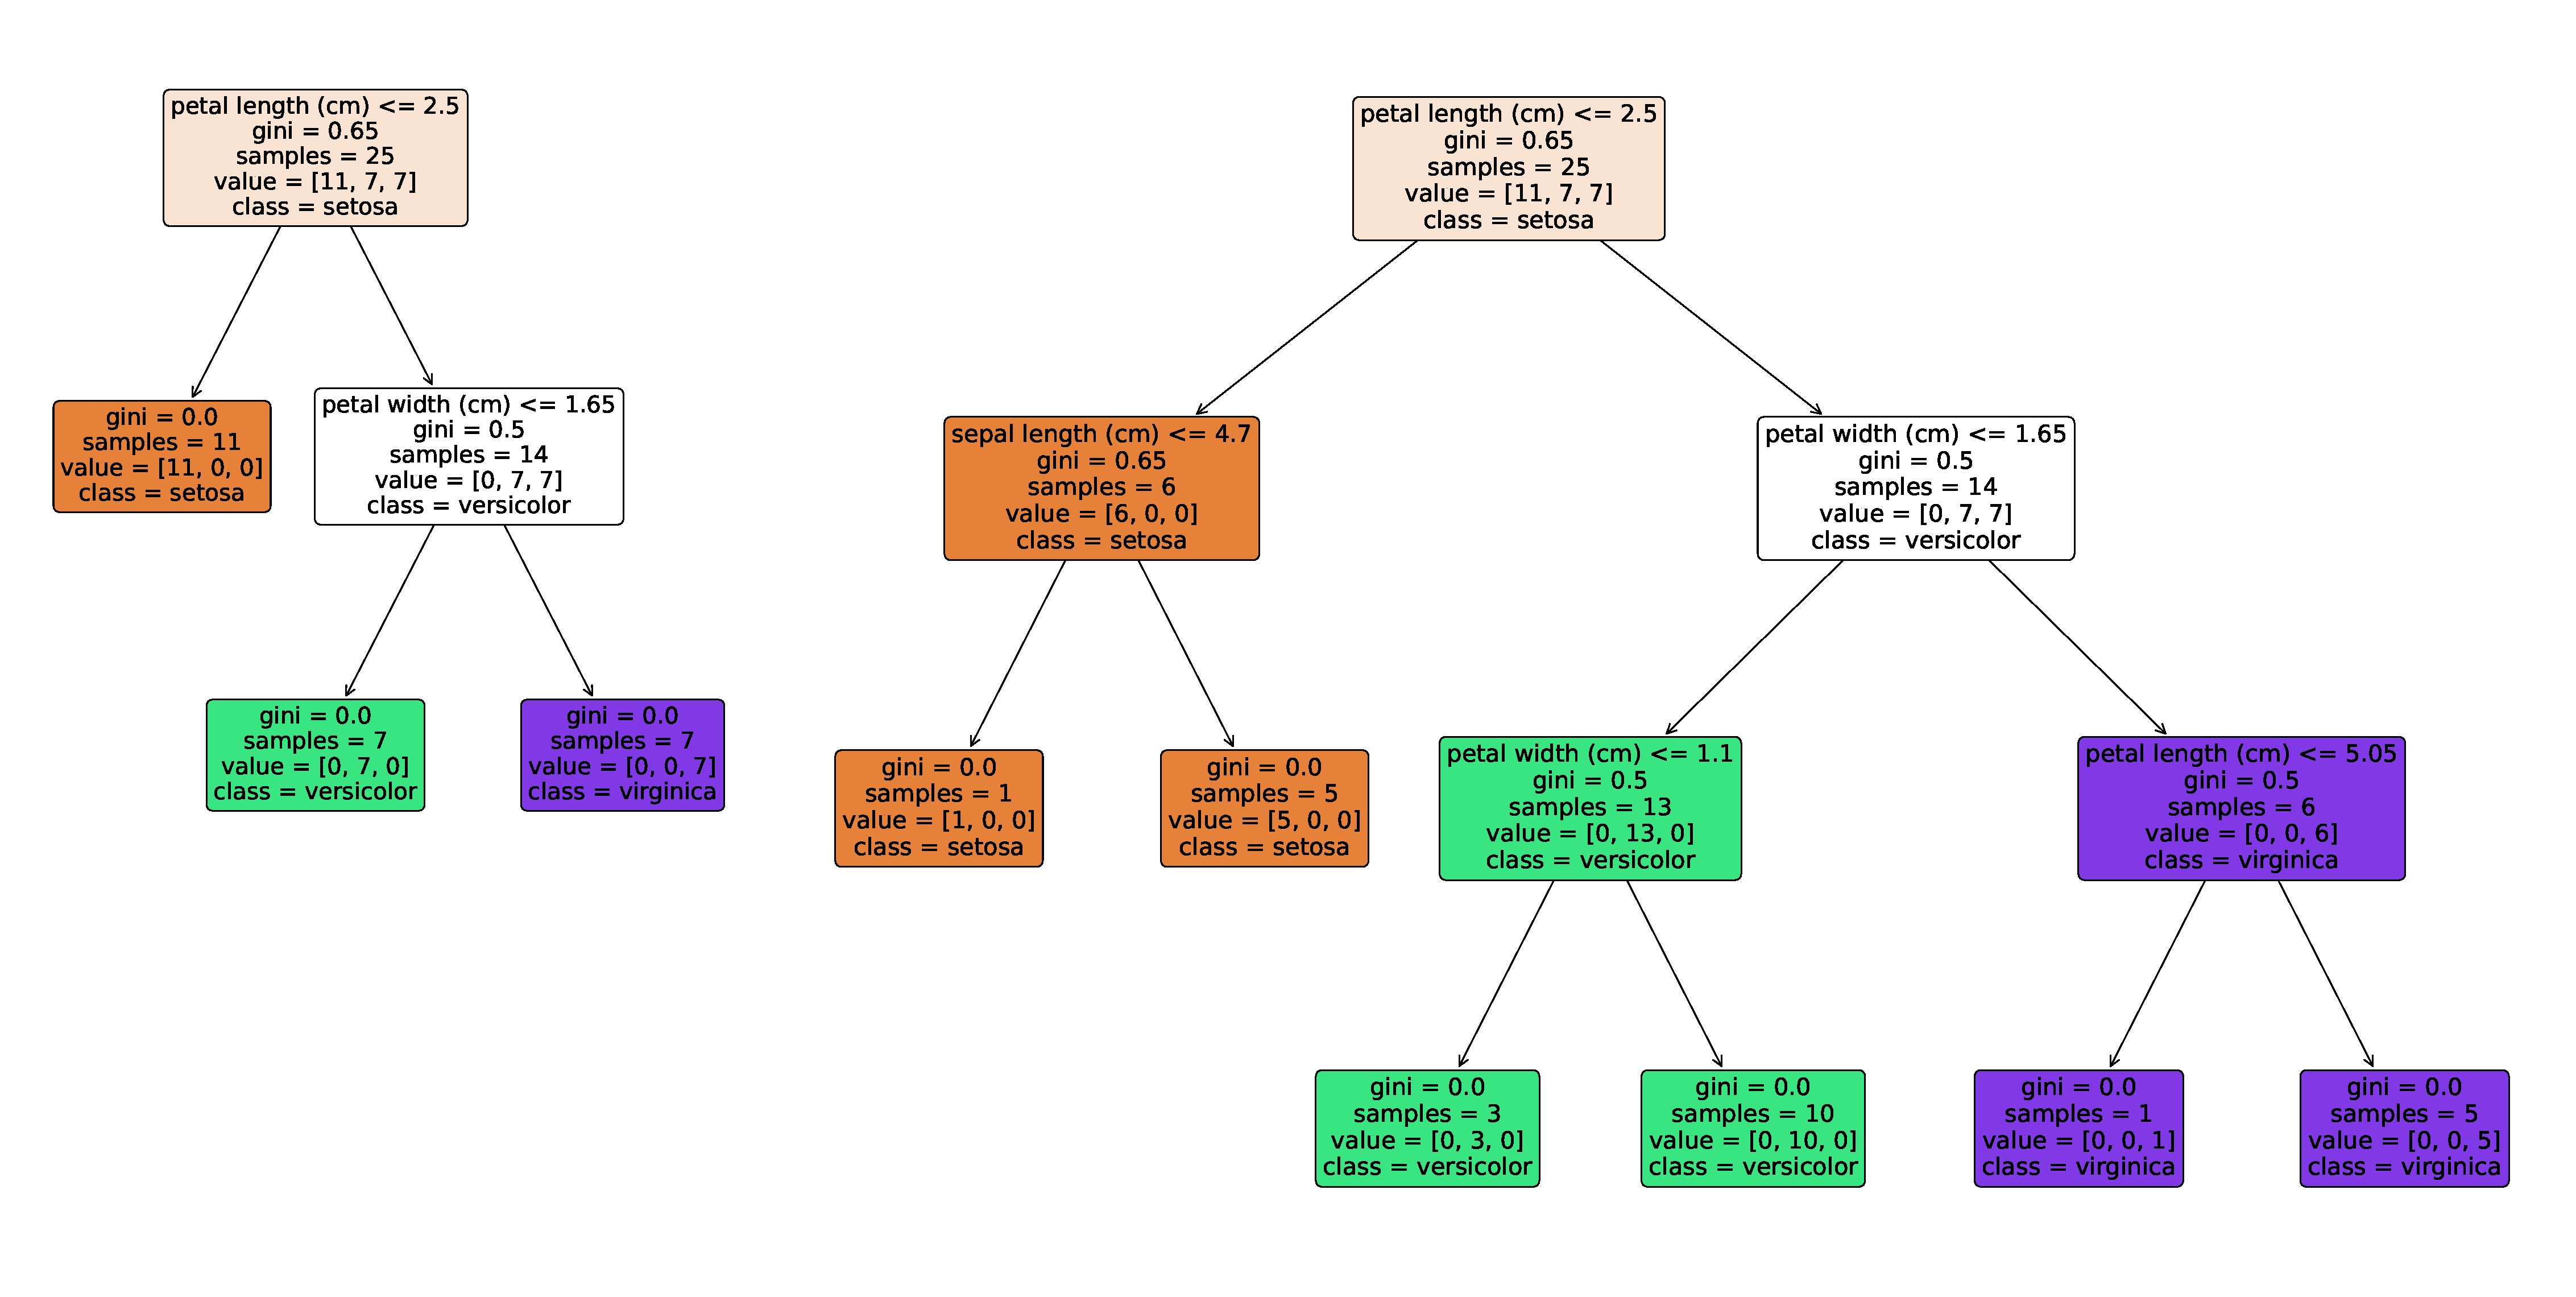
\includegraphics[width=\textwidth]{iris}
  \caption{A Stream Decision Tree on the Iris dataset after the first data batch \textbf{(left)} and the second data batch \textbf{(right)}. The algorithm takes the three leaf nodes \textbf{(left)} and splits them with respect to the second data batch. The internal nodes are never modified, preserving earlier partitions of the feature space.
  }
\label{fig:iris}
\end{figure*}

\begin{algorithm}[!htb]
\caption{Incrementally update a decision forest with a batch of training samples.}
\label{alg:sdf}
\begin{algorithmic}[1]
\Require
\Statex (1) $\mathbf{T}$ \Comment{current forest}
\Statex (2) $\mathcal{D}_n = (\mathbf{x},\mathbf{y}) \in \mathbb{R}^{n \times p} \times \{1,\ldots, K\}^n$ \Comment{batch of training samples}
\Statex (3) split criteria \Comment{e.g., minimum node size}
\Statex (4) $r$ \Comment{number of trees to replace}
\Ensure
$\mathbf{T}$ \Comment{updated forest}
\Function{SDF.update\_forest}{$\mathbf{T},\mathbf{x},\mathbf{y},r$}
\For{each each tree in the forest}
\State resample ($\mathbf{x},\mathbf{y}$) with bootstrapping
\State limit the number of features used for splitting
\State update the tree with resampled data 
\EndFor
\State record $b$, the number of batches seen
\If{$b$ is greater than 1}
with $1/b$ probability:
\State find the accuracy of trees with respect to the current batch
\State sort the indices of worst performing trees
\For{each $i \in [r]$}
\State resample ($\mathbf{x},\mathbf{y}$) with bootstrapping
\State create a new tree with resampled data
\State replace an old tree with the new tree 
\EndFor
\EndIf
\State \Return $\mathbf{T}$
\EndFunction
\end{algorithmic}
\end{algorithm}

SDTs are based on a fork of the scikit-learn python package (BSD-3-Clause), which we customized by adding a new \texttt{partial\_fit} function to \texttt{DecisionTreeClassifier} for extending fitted trees \citep{pedregosa_scikit-learn_2011}. Thus, an SDT is initialized almost in the same way as a DT, where the tree is fitted to the first batch of training samples. The only difference is the input of predefined class labels, as the first batch might not include all possible classes. 
For each incremental update afterwards (Algorithm \ref{alg:sdt}), the SDT takes in one batch of training samples: $\mathcal{D}_n = (\mathbf{x},\mathbf{y}) \in \mathbb{R}^{n \times p} \times \{1,\ldots, K\}^n$. 
Then for every training sample $x_i$ in the batch, the algorithm locates the leaf node it would fall into and associates the node with the sample. All the leaf nodes found in such a manner are marked as ``false roots.'' 
These ``false roots'' are then split and extended if satisfying the prespecified splitting criteria (e.g. a minimum node sample size of two). 
If the splitting occurs, both child nodes would be recursively marked as ``false roots'' and associated with their separate training samples, just like how batch splitting works in DTs. If not fulfilling the splitting criteria, the ``false roots'' would become the new leaf nodes. Figure \ref{fig:iris} shows an example of SDT structures on the Iris dataset \citep{fisher_uci_1988}. Two random batches of 25 samples were used.

An SDF, defined as \texttt{StreamDecisionForest} 
\footnote{\url{https://sdtf.neurodata.io/}}
in code, is initialized as a collection of SDTs (100 by default) and modeled after scikit-learn's RF implementation: \texttt{RandomForestClassifier} \citep{pedregosa_scikit-learn_2011}. As in Algorithm \ref{alg:sdf}, it incrementally updates the trees by bootstrapping the training batches and limiting the number of features selected per split (``max\_features''). The default ``max\_features'' is defined as $\sqrt{d}$, where $d$ is the total number of features. After each incremental update, with $1/b$ probability, where $b$ is the number of batches seen, the forest replaces its worst performing trees (one tree by default) with new trees fitted only to the current batch. We include the probability aspect to uniformly sample over the training sets and thus minimize the bias towards the most recent data. This step removes SDTs that are negatively affected by earlier partitions and reduces the computational space taken. All predictions are generated via majority voting, which helps improving the ensemble's consistency \citep{liaw_classification_2002, biau_consistency_2008, breiman_random_2001}. Furthermore, the algorithm uses the joblib python package (BSD-3-Clause) and takes advantage of parallel computing \citep{joblib_developers_joblibjoblib_2022}.

In all benchmarks, we incrementally updated SDTs and SDFs with fixed-sized training batches (100 random samples per batch) and measured their performance on separated test sets.

\subsection{Reference Algorithms}
For comparison with state-of-the-art streaming tree algorithms, we experimented with two existing estimators: Hoeffding trees and Mondrian forests \citep{domingos_mining_2000, lakshminarayanan_mondrian_2014, khannouz_benchmark_2020, pfahringer_new_2007, gomes_machine_2019, lakshminarayanan_mondrian_2016}. 

HTs, also known as VFDTs (Very Fast Decision Trees), are designed to grow tree learners incrementally using Hoeffding bounds \citep{domingos_mining_2000, hoeffding_probability_1994}. 
After observing $n$ samples within range $R$, the bound states that, with $1 - \delta$ probability, the variable's true mean is no smaller than the sample mean minus $\epsilon$, where 
\begin{equation*} \epsilon=\sqrt{\frac{R^2\ln(\delta^{-1})}{2n}} \tag{1} \end{equation*}
Thus, the algorithm's robustness is determined by specifying the $\delta$ value.
This statistical bound is independent of heuristic measures (e.g. Gini index and information gain), and the tree splits the current leaf node after observing enough samples.

When training with large datasets, HTs could take up excessive memories to account for all growing leaves \citep{domingos_mining_2000, lavanya_handwritten_2017}. Thus, resource constraints would temporarily deactivate low performing leaves and reactivate them as needed. The algorithm constantly monitors the error rates of all leaf nodes and the probabilities of samples falling into them. 
For experiments, we used \texttt{HoeffdingTreeClassifier} from the river python package (BSD-3-Clause) \citep{montiel_river_2020}. The max size of HTs was set as 1,000 MB, and the minimum sample size for splitting (``grace\_period'') was changed to two.

On the other hand, MFs utilize Mondrian processes to incrementally grow Mondrian trees, which are named after Piet Mondrian's paintings (e.g. Figure \ref{fig:mondrian_paint}) \citep{lakshminarayanan_mondrian_2014, roy_mondrian_2009, mondrian_dutch_1921}. The Mondrian processes recursively construct random and hierarchical partitions in the feature space. They assign probabilities in a consistent way, and new splits cannot intercept the existing splits \citep{lakshminarayanan_mondrian_2014}. Specifically in the one-dimensional case, the partitions are shown to be a Poisson point process \citep{roy_mondrian_2009}. The forests utilize up to three types of operations when introducing a new sample: splitting existing leaves, updating existing partitions, and creating new splits from internal nodes \citep{lakshminarayanan_mondrian_2014}.
We used \texttt{MondrianForestClassifier} from the scikit-garden python package (BSD-3-Clause) \citep{kumar_scikit-gardenscikit-garden_2017}. The default total number of estimators (``n\_estimators'' = 10) must be used to ensure enough computational space, which is further explored in Section \ref{results:select}.

\begin{figure}[!htb]
\centering
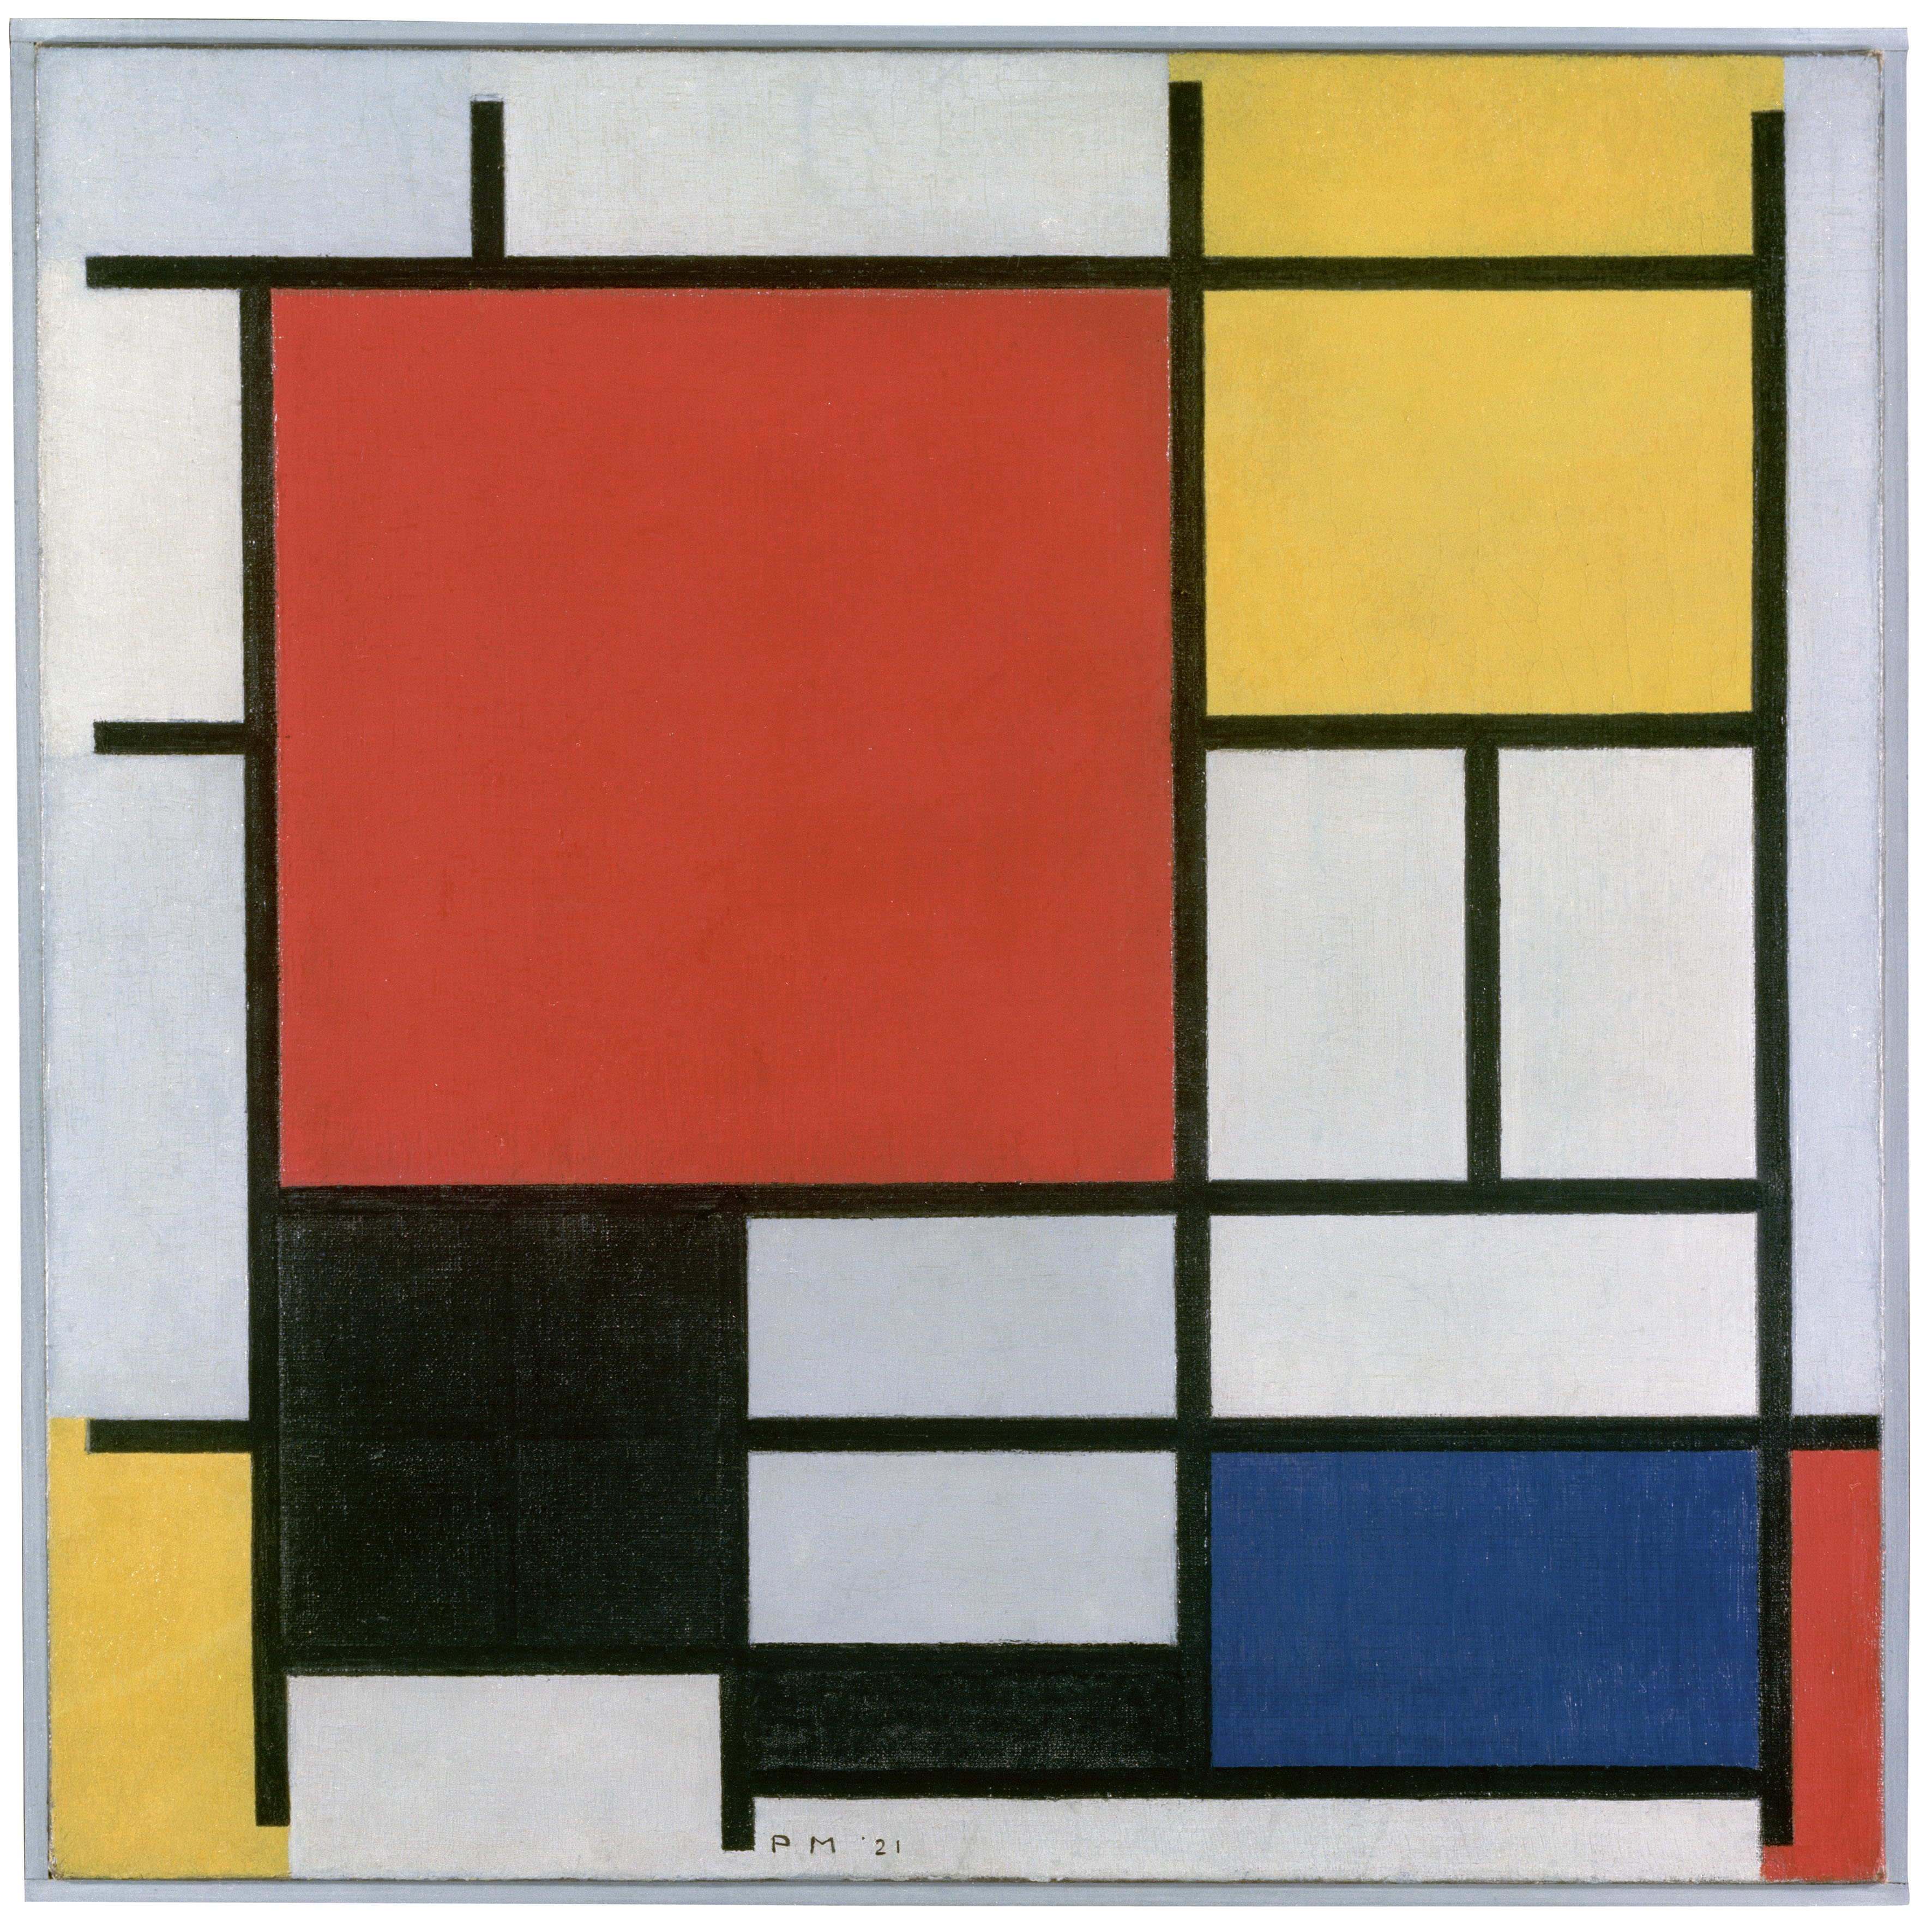
\includegraphics[width=0.3\columnwidth]{mondrian_paint.jpeg}
  \caption{\textit{Composition with Red, Yellow, Blue, and Black} by Piet Mondrian (1921).
  }
\label{fig:mondrian_paint}
\end{figure}

For comparison with batch tree estimators, we included batch decision trees and random forests \citep{breiman_random_2001}. An RF contains a collection of DTs (100 by default) and uses bootstrapping to resample the training data. Each tree in the forest limits the number of features selected at each node split (``max\_features'') and tries to find the best partitions available \citep{breiman_random_2001}.
With majority voting as predictions, an RF is non-parametric and universally consistent, so it will approach Bayes optimal performance with sufficiently large sample sizes, tree depths, and number of trees \citep{liaw_classification_2002, biau_consistency_2008}.
Implementations for both algorithms were from the scikit-learn package: \texttt{DecisionTreeClassifier} and \texttt{RandomForestClassifier} \citep{pedregosa_scikit-learn_2011}. All hyperparameters were kept as default.

In all tasks, we incrementally updated HTs and MFs with fixed-sized data batches (100 random samples per batch). At each sample size, DTs and RFs were trained with all available data, including current and previous batches. 

\subsection{Data}
We selected three standard datasets (Table \ref{table:data}) for experiments: Splice-junction Gene Sequences (Splice), Pen-Based Recognition of Handwritten Digits (Pendigits), and CIFAR-10 \citep{towell_molecular_1991, alpaydin_pen-based_1998, krizhevsky_learning_2012, lavanya_handwritten_2017}.

For the Splice dataset, we randomly reserved 25\% of all genetic sequences for testing \citep{rampone_splice-junction_1998, sarkar_splice_2020}. Each sequence contains 60 nucleotide codes, which are converted into numerical features by the OpenML curation \citep{feurer_openml-python_2019}. This task tests MFs' performance on DNA data without feature engineering, which was not satisfactory in the original paper \cite{lakshminarayanan_mondrian_2014}. 
The Pendigits dataset contains handwritten images represented by 16 pixel features, which are generated through spatial resampling \citep{alimoglu_methods_1996}.
The CIFAR-10 dataset contains RGB-colored images, each high-dimensional image represented by $32 \times 32 \times 3 = 3,072$ pixel features. We used the provided training and test sets for Pendigits and CIFAR-10, and ran the three tasks 10 times by randomizing the training sets. Excessive memory requirements of MFs prevented us from conducting cross validations.

\begin{table}[htb]
\centering
\begin{tabular}{lccc} 
\hline
Dataset & \textbf{Splice} & \textbf{Pendigits} & \textbf{CIFAR-10} \\
\hline
\# Features & $60$ & $16$ & $3,072$ \\
\hline
\# Classes & $3$ & $10$ & $10$ \\
\hline
\# Train & $2,392$ & $7,494$ & $50,000$ \\
\hline
\# Test & $798$ & $3,498$ & $10,000$ \\
\hline
\end{tabular}
\caption{Dataset attributes for three selected tasks.}
\label{table:data}
\end{table}

We also used the OpenML-CC18 data suite for further benchmarks on SDFs and RFs. It represents a collection of 72 real-world datasets organized by OpenML and functions as a comprehensive benchmark suite \citep{vanschoren_openml_2013, bischl_openml_2019}. These datasets vary in sample size, feature space, and unique target classes.
About half of the tasks are binary classifications, and the other half are multiclass classifications with up to 50 classes. The range of total sample sizes is between 500 and 100,000, while the range of features is from a few to a few thousand \citep{bischl_openml_2019}.
Datasets were imported using the OpenML-Python package (BSD-3-Clause) \citep{feurer_openml-python_2019}. In the OpenML-CC18 tasks, We used all available samples and ran 5-fold cross validations with SDFs and RFs.

\subsection{Evaluation Metrics}
Classifier performance is evaluated by classification accuracy, virtual memories, and training wall times. 
On the three selected datasets, we use the psutil python package (BSD-3-Clause) to measure memory usage from the first repetitions
% , which doesn't account for pinned and anonymous pages 
\citep{rodola_giampaolopsutil_2022}.
The training wall times calculate the fitting times for the given model without hyperparameter tuning. All estimators' times are calculated by accumulating the training times of data batches, which account for batch estimators' refitting. We do not report any error bars as they are uninformative. 
To accommodate the space and time constraints of MFs and HTs, the three selected tasks were run without parallelization on a Microsoft Azure 6-core (Intel Xeon E5-2690 v3) Standard\_NC6 instance with 56 GB memory and 340 GB SSD storage.
The OpenML-CC18 experiments were run with parallelization on a Microsoft Azure 4-core (Intel Xeon E5-2673 v4) Standard\_D4\_v3 instance with 16 GB memory and 100 GB SSD storage.

\begin{figure*}[!htb]
\centering
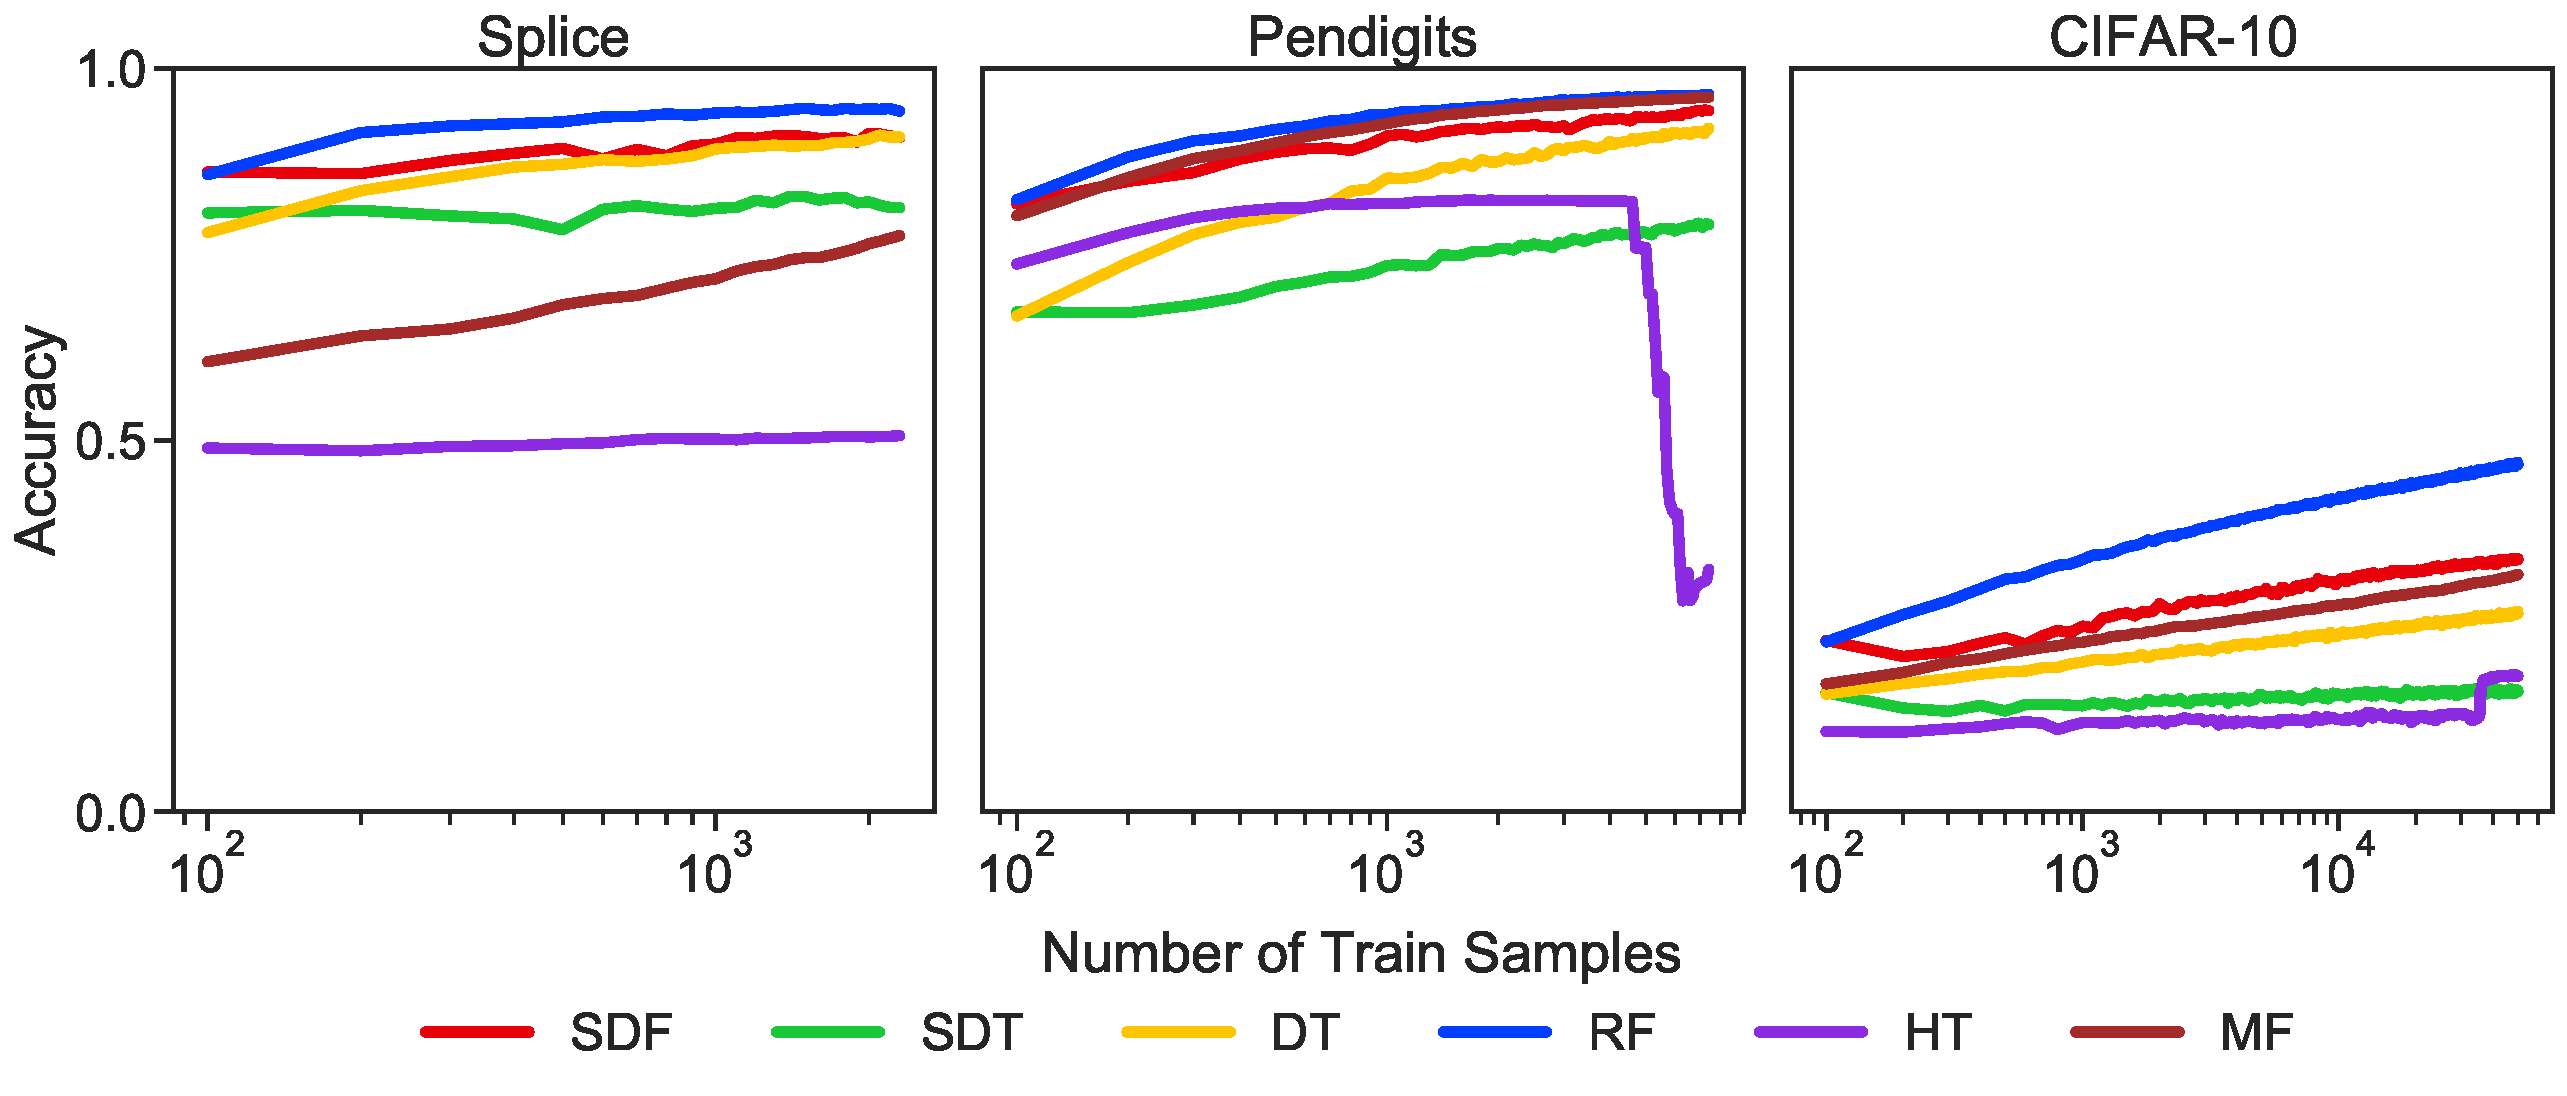
\includegraphics[width=0.9\textwidth]{select_acc}
  \caption{Multiclass classifications on the Splice \textbf{(left)}, Pendigits \textbf{(center)}, and CIFAR-10 \textbf{(right)} datasets. 
  Each line represents averaged results from 10 randomized repetitions. Stream Decision Forests (SDFs) perform better than all other streaming estimators on the Splice and CIFAR-10 datasets. They also perform very similarly to Mondrian forests (MFs) and random forests (RFs) in the Pendigits task. The performance of Hoeffding trees (HTs) either remains almost constant or experiences significant fluctuations. Especially in the Pendigits task, the accuracy drops continuously from around 4,000 samples to about 6,000 samples. MFs perform as best as RFs in the Pendigits task, but their accuracy significantly drops in the Splice task, only surpassing that of HTs. Batch decision trees (DTs) perform consistently in all tasks.
  }
\label{fig:select_acc}
\end{figure*}

\section{Results}
\label{results}

\subsection{Three Selected Tasks}
\label{results:select}
SDFs achieve consistently high accuracy across all sample sizes and classification tasks, as compared to MFs and HTs. Specifically in the Splice and CIFAR-10 tasks (Figure \ref{fig:select_acc}, left and right), the algorithm always performs the best among streaming classifiers. Its accuracy is also very close to the highest on the Pendigits dataset (Figure \ref{fig:select_acc}, center). 
The performance of single SDTs shows substantial increase in the Pendigits task (Figure \ref{fig:select_acc}, center). 
These results clearly illustrate that our streaming trees and ensembles incrementally optimize the tree structures with new information, benefiting from continual data batches.

HTs always have the lowest accuracy when training on the Splice dataset, which remains almost constant as sample size increases (Figure \ref{fig:select_acc}, left). In this case, the classifier fails to learn any new information from continual data batches.
It also shows performance fluctuations when training on the other two datasets. In the Pendigits task, the accuracy starts dropping significantly around 4,000 samples until rebounding at 6,000 samples (Figure \ref{fig:select_acc}, center). In the CIFAR-10 task, there is a sudden performance increase around 32,000 samples, barely overtaking the accuracy of SDTs (Figure \ref{fig:select_acc}, right).
We speculate that the fluctuations are related to how the algorithm regulates low performing leaves under resource constraints \citep{domingos_mining_2000}. However, our attempts of increasing the maximum size of HTs, even to excessive amounts beyond the memory limits, would not alleviate the problem. 
Such disadvantages could prevent HTs from producing meaningful results on certain datasets or maintaining consistent performance at larger samples sizes.

In the Pendigits task, MFs perform as good as RFs at larger sample sizes (Figure \ref{fig:select_acc}, center). However, their accuracy is even worse than batch DTs' on the Splice dataset, only surpassing the almost constant plots of HTs (Figure \ref{fig:select_acc}, left). 
We find MFs' worse performance in the Splice task as expected due to previous experiments on DNA data \citep{lakshminarayanan_mondrian_2014}. 
The accuracy could be improved if feature engineering is implemented, demonstrating the drawbacks of label-independent random splits on certain data domains \citep{roy_mondrian_2009, ziegler_mining_2014}.
Moreover, MFs perform worse than SDFs on the CIFAR-10 dataset (Figure \ref{fig:select_acc}, right). The results show that SDFs are better at handling more feature dimensions.

\begin{figure}[!htb]
\centering
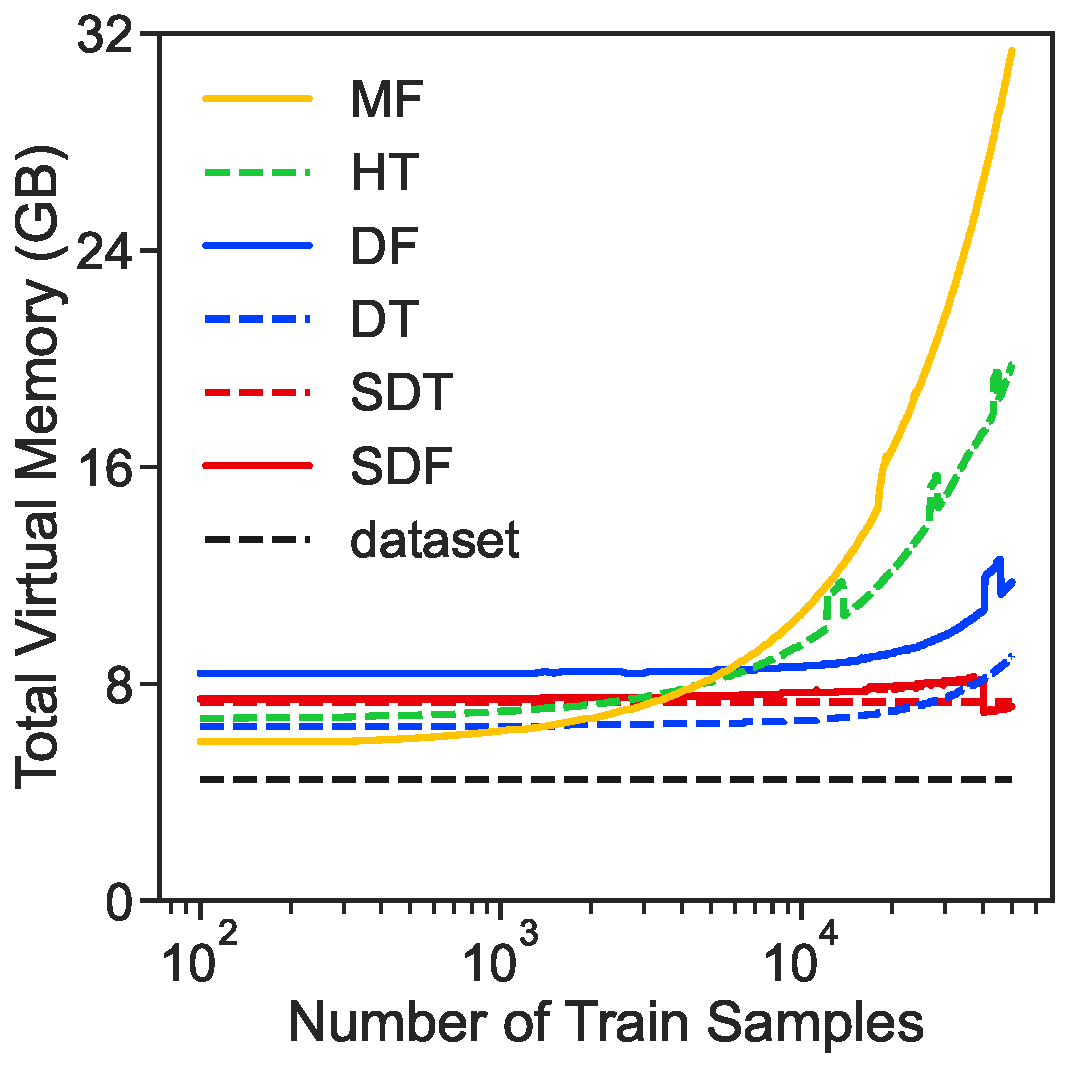
\includegraphics[width=0.4\columnwidth]{select_cifar_mem}
  \caption{Multiclass classifications on the CIFAR-10 dataset. Each solid line shows the classifier's virtual memories during the first repetition, and the dashed line shows the memory taken by loading the CIFAR-10 dataset and packages. The classifiers are ordered by their memory usage at the largest sample size. At the largest sample size, Stream Decision Forests (SDFs) are the most space efficient, and the usage decrease at 40,000 samples could be attributed to the algorithm's tree replacements. Hoeffding trees (HTs) and Mondrian forests (MFs) take up excessive memories as sample size increases.
  }
\label{fig:select_cifar_mem}
\end{figure}

In terms of computational space, SDFs are the most efficient on the CIFAR-10 dataset at the largest sample size (Figure \ref{fig:select_cifar_mem}). The classifier's memory usage drops substantially around 40,000 samples, which could be attributed to its tree replacement approach (Algorithm \ref{alg:sdf}). SDTs have the second lowest memory usage, and both algorithms use less than batch DTs and RFs. However, the other two streaming classifiers: HTs and MFs both take up excessive virtual memories as sample size increases. At the maximum sample size, an HT has more than quadrupled the memory required by the dataset and packages (4.5 GB), and an MF even occupies more than 30 GB of computational space. Such space constraints significantly limit these two algorithms' applications, and the total number of trees in MFs must be restricted to ensure task completion. 
Thus, SDFs would be considered the optimal choice for streaming tasks with limited resources. We do not report the other two tasks' virtual memories as the changes are minimal. See Appendix \ref{app:select_time} for results on training wall times.

\begin{figure}[!htpb]
\centering
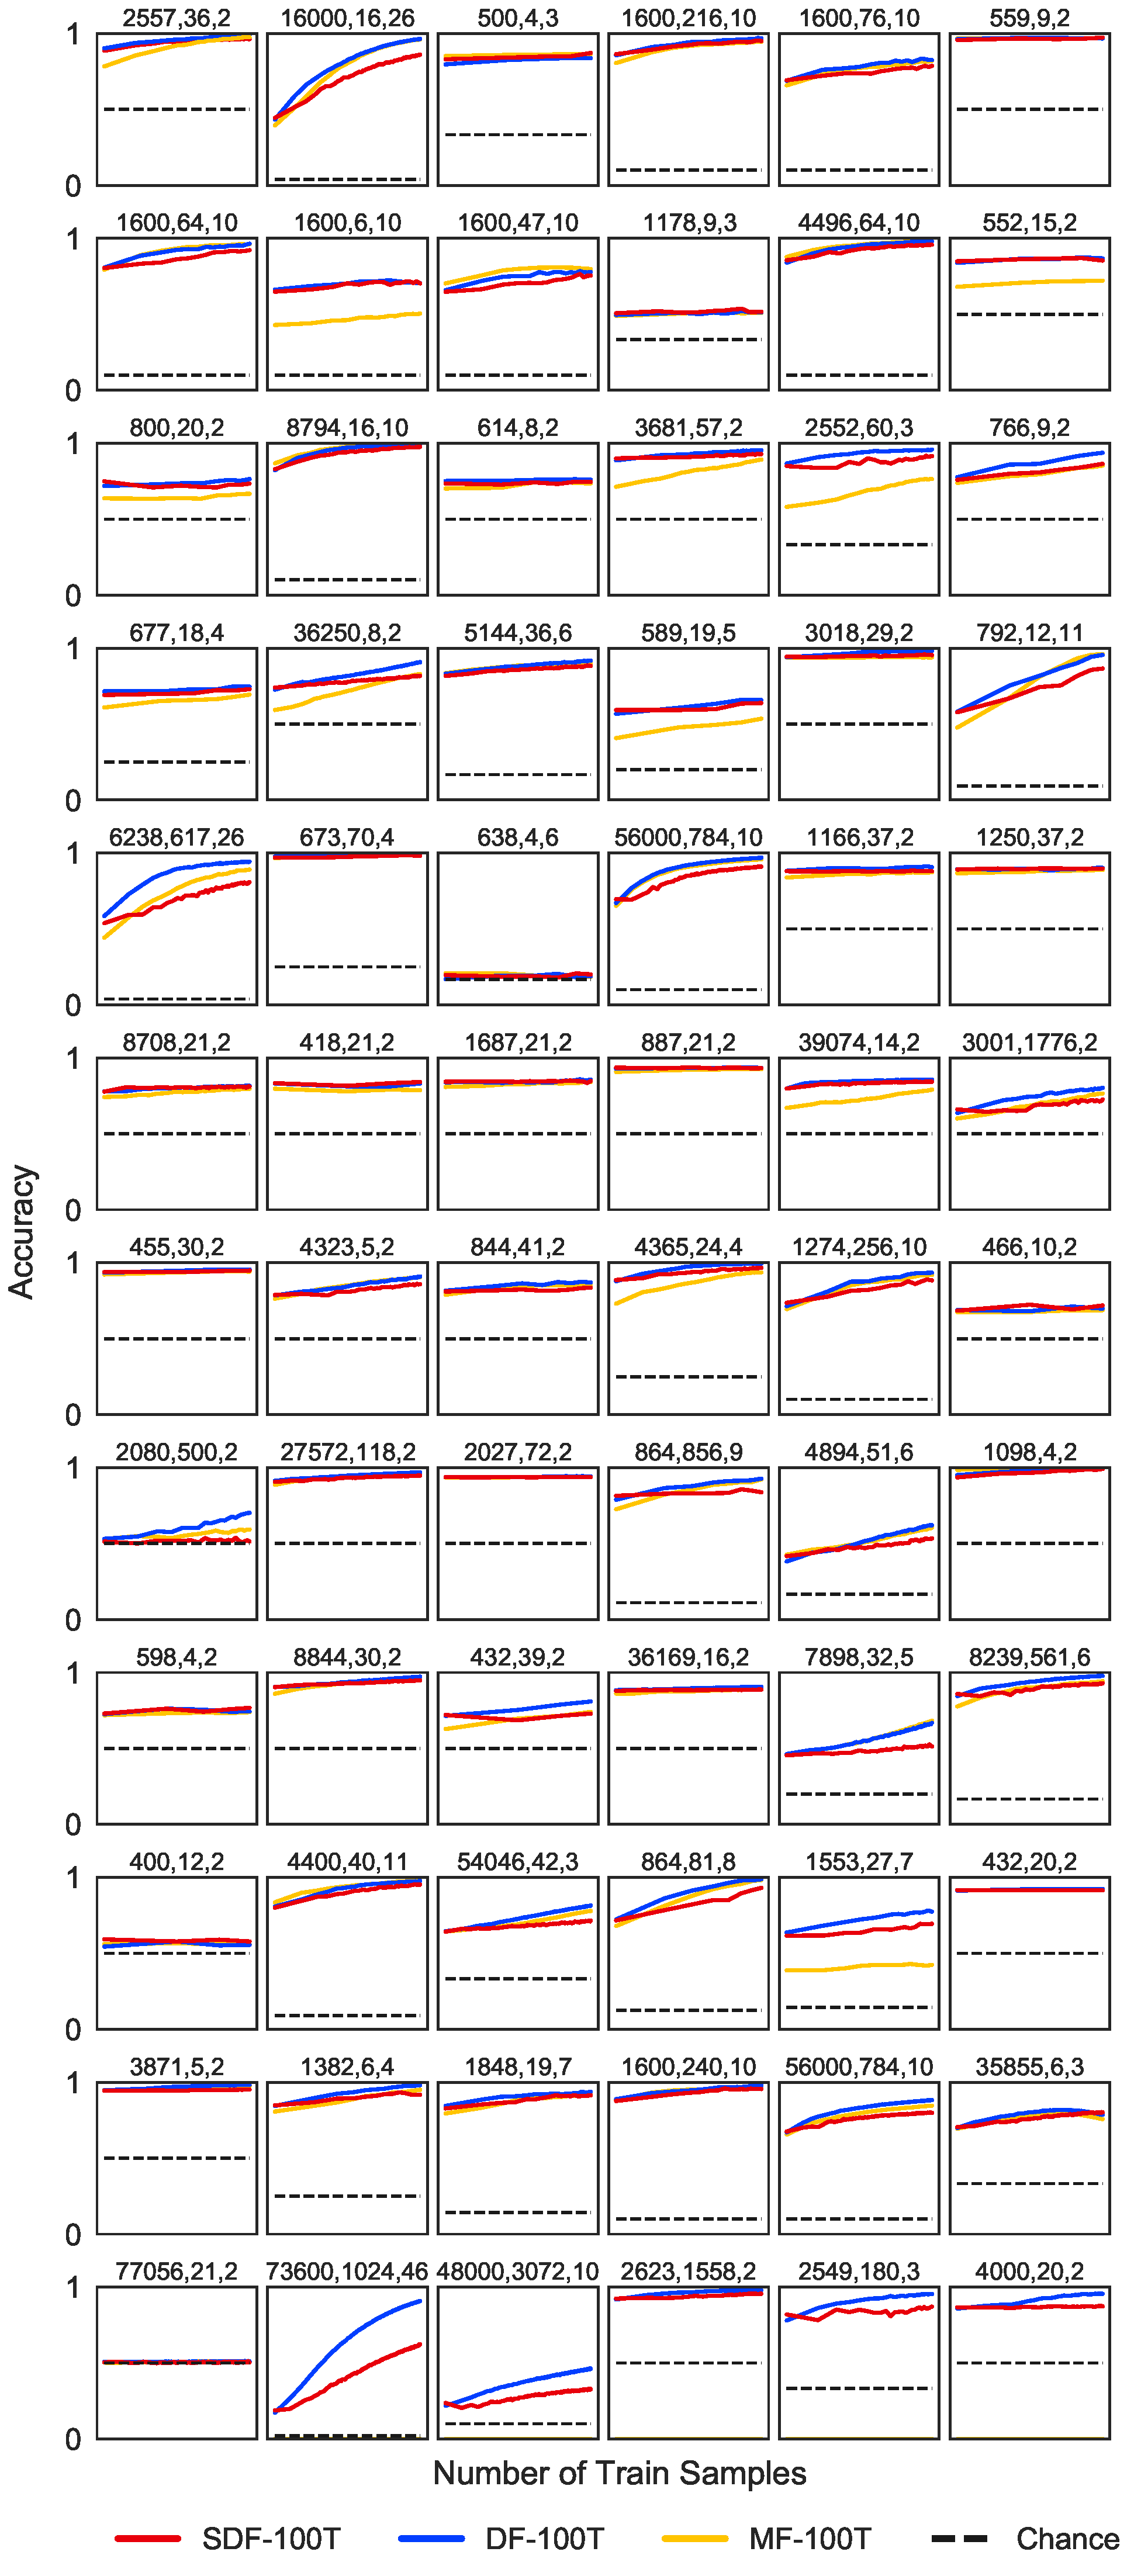
\includegraphics[width=0.5\columnwidth]{cc18}
  \caption{Classifications on the OpenML-CC18 datasets. All plots show averaged accuracy over five folds and have dataset IDs as titles. In many tasks, Stream Decision Forests (SDFs) perform as good, sometimes even better, than random forests (RFs). Moreover, SDF accuracy consistently increases with new data. This consistency across different data domains makes SDFs more applicable to real-world problems than other streaming tree algorithms.
  }
\label{fig:cc18}
\end{figure}

\subsection{OpenML-CC18 Tasks}
In the OpenML-CC18 tasks, SDFs show high classification accuracy and consistent improvements as more data batches come in. They often achieve performance as well, sometimes even better, than that of RFs (Figure \ref{fig:cc18}). These results illustrate that the ensemble can maintain its performance on datasets across a variety of data domains, including tabular, images, audios, and more \citep{bischl_openml_2019}. Such consistency makes SDFs applicable to diverse real-world scenarios, avoiding the disadvantages of HTs and MFs.

\begin{figure}[!htb]
\centering
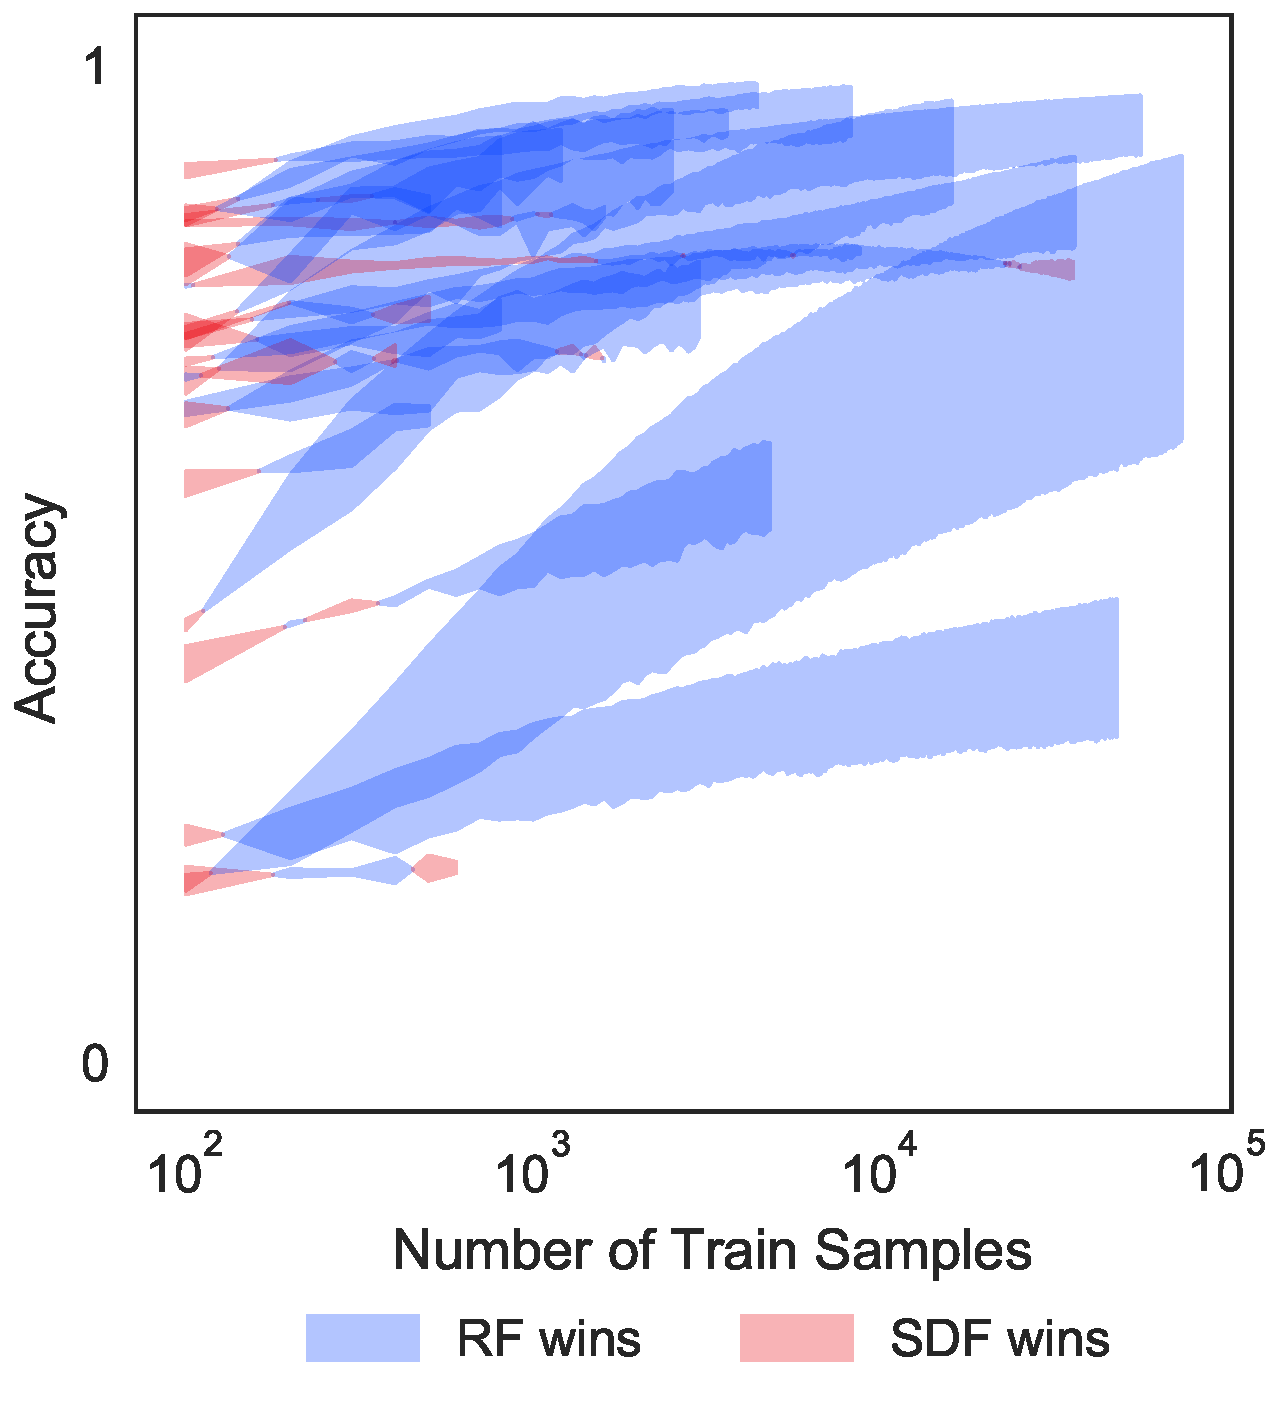
\includegraphics[width=0.4\columnwidth]{cc18_fill}
  \caption{Classifications on the OpenML-CC18 datasets with substantial effect size shifts (minimum $\leq -1\%$ and maximum $\geq 1\%$). Each filled area represents average accuracy from 5-fold cross validations in one classification task. Red blocks show the better performance of Stream Decision Forests (SDFs), while blue blocks show the better performance of random forests (RFs). SDFs would perform better than RFs at smaller sample sizes, and this advantage persists longer in less complex tasks (high accuracy at small sample sizes).
  }
\label{fig:cc18_fill}
\end{figure}

We calculate the effect sizes by averaging the classification accuracy across five folds and measuring the difference ratios:
\begin{equation*} \frac{\overline{SDF} - \overline{RF}}{\overline{RF}} \tag{2} \end{equation*}
Positive percentages represent the better performance of SDFs, while negative values represent that of RFs. 
As sample size increases, certain tasks show substantial shifts of effect size (Figure \ref{fig:cc18_fill}), which has a minimum $\leq -1\%$ and a maximum $\geq 1\%$. 
On these datasets, SDFs usually perform better than RFs at smaller sample sizes. The persistence of such an advantage would depend on the datasets' complexities; tasks with high accuracy at small sample sizes maintain the SDF dominance longer. In other words, having more data available allows batch RFs to achieve better performance on more difficult datasets. 
However, this scenario is unreasonable in real-world applications, and refitting batch RFs at large sample sizes demands much more computational resources than incrementally updating SDFs (Figure \ref{fig:select_cifar_mem}).

In conclusion, we demonstrate that our algorithms, the simplest approach to streaming trees and ensembles, achieve consistently high performance on a variety of real-world datasets. 
We also illustrate that SDFs avoid the current problems of HTs and MFs, which perform catastrophically on certain datasets and take up excessive memories at large sample sizes. 

\section{Discussion}
\label{discussion}
Our streaming tree algorithms: SDTs and SDFs utilize the simplest strategy of extending fitted decision trees (Algorithm \ref{alg:sdt} and \ref{alg:sdf}). It maintains all the existing partitions and further splits the feature space with new data batches (Figure \ref{fig:iris}). This approach is easier to implement than Hoeffding bounds and Mondrian processes, as both methods modify the tree splitting mechanisms \citep{hoeffding_probability_1994, domingos_mining_2000, roy_mondrian_2009, lakshminarayanan_mondrian_2014}. 
Furthermore, SDFs achieve consistently high accuracy in diverse classification tasks and often perform as well, occasionally even better, than state-of-the-art batch RFs (Figure \ref{fig:select_acc} and \ref{fig:cc18}). These results show that our methods avoid the problems of HTs and MFs, which perform poorly in some tasks and occupy huge amounts of memory in others (Figure \ref{fig:select_acc} and \ref{fig:select_cifar_mem}). Thus, SDTs and SDFs establish a simple standard for streaming trees that could be readily applied to many real-world problems.

On some datasets with high complexities, batch trees and ensembles could achieve more accurate results if all samples are given at once (Figure \ref{fig:cc18} and \ref{fig:cc18_fill}). Nonetheless, this assumption is very unlikely in real-world scenarios \citep{abdulsalam_streaming_2007, liu_isolation_2008}. In our experiments and actual practices, batch decision trees and forests need to store all available data and refit themselves every time a new batch of samples comes in. Even by restricting the number of refitting with certain criteria (e.g. a minimum amount of new samples), it would still cost significantly more computational resources than incremental updates (Figure \ref{fig:select_cifar_mem}). Thus, our streaming trees provide an alternative solution to such tasks. As an SDF continuously improves its partitions with new information, any differences in performance would eventually be eliminated by enough data batches. It is therefore more economical to keep updating an established streaming model than constructing a new batch forest from time to time.

Although our experiments focus on one in-distribution task, SDFs' applications could be extended to solve OOD problems like distribution shift and continual learning \citep{geisa_towards_2021, van_de_ven_three_2019}. 
Technically, each extension of decision trees does not have to rely on samples from the same distribution or use the same splitting criteria. Old trees can also be replaced anytime if previous partitions fail to perform well on current data streams. 
Moreover, as supplemental data arrive, continual learning models could leverage SDFs to incrementally update existing tasks.

Overall, our method of incremental updates excels at simplicity, consistency, space efficiency, and extensibility. This approach could offer great development potentials and set a clear standard for streaming tree algorithms, focusing on real-world applications.